% ============================================================
%  يُترجَم بـ XeLaTeX  (في Overleaf: Menu → Compiler → XeLaTeX)
%  الخط: Amiri (متوفر في Overleaf، أو حمّله من github.com/aliftype/amiri)
% ============================================================
\documentclass[12pt,a4paper]{article}
\usepackage[a4paper,margin=1.7cm,top=2.3cm,bottom=2.9cm,headheight=15pt,footskip=1.5cm]{geometry}
\usepackage{amsmath,amssymb}
\usepackage{icomma}
\usepackage[english,bidi=default,layout=lists]{babel}
\babelprovide[import,main]{arabic}
\babelfont{rm}[Scale=1.08]{Amiri}
\babelfont{sf}[Scale=1.08]{Amiri}
\usepackage[most]{tcolorbox}
\usepackage{tikz}
\usetikzlibrary{arrows.meta,calc,shadings}
\usepackage{array}
\usepackage{colortbl}
\usepackage{fancyhdr}
\usepackage{titlesec}
\usepackage{enumitem}
\usepackage{collcell}
\usepackage{needspace}
\usepackage{etoolbox}
\newcolumntype{C}{>{\collectcell\ar}c<{\endcollectcell}}
\pretocmd{\section}{\Needspace{15\baselineskip}}{}{}
\pretocmd{\subsection}{\Needspace{11\baselineskip}}{}{}

\definecolor{cDef}{HTML}{1F4E9C}
\definecolor{cThm}{HTML}{B3261E}
\definecolor{cRem}{HTML}{2E7D32}
\definecolor{cEx}{HTML}{C76B00}
\definecolor{cMeth}{HTML}{6A1B9A}
\definecolor{cSol}{HTML}{00695C}
\definecolor{cSec}{HTML}{1F3A68}

\titleformat{\section}{\Large\bfseries\color{cSec}}{\thesection.}{0.6em}{}[{\color{cSec!60}\titlerule[1pt]}]
\titleformat{\subsection}{\large\bfseries\color{cThm!85!black}}{\thesubsection.}{0.5em}{}
\titlespacing*{\section}{0pt}{14pt}{8pt}
\titlespacing*{\subsection}{0pt}{10pt}{5pt}
\setlength{\parindent}{0pt}
\setlength{\parskip}{4pt}
\setlist{itemsep=2pt,topsep=3pt}

\newtcolorbox{arbox}[3][]{enhanced,
  colback=#2!5,colframe=#2!80!black,arc=2mm,boxrule=0.8pt,
  left=6pt,right=6pt,top=8pt,bottom=5pt,
  fonttitle=\bfseries,coltitle=white,
  title={\foreignlanguage{arabic}{#3}},
  attach boxed title to top right={xshift=-5mm,yshift=-3mm},
  boxed title style={colback=#2!80!black,arc=1.5mm,boxrule=0pt},
  before upper={\selectlanguage{arabic}},
  before skip=8pt,after skip=8pt,breakable,#1}
\newenvironment{BOX}[2]{\begin{otherlanguage}{english}\begin{arbox}{#1}{#2}}{\end{arbox}\end{otherlanguage}}
\newenvironment{tarif}[1][تعريف]{\begin{BOX}{cDef}{#1}}{\end{BOX}}
\newenvironment{khassia}[1][خاصية]{\begin{BOX}{cThm}{#1}}{\end{BOX}}
\newenvironment{molahada}[1][ملاحظة]{\begin{BOX}{cRem}{#1}}{\end{BOX}}
\newenvironment{mithal}[1][مثال]{\begin{BOX}{cEx}{#1}}{\end{BOX}}
\newenvironment{tariqa}[1][طريقة]{\begin{BOX}{cMeth}{#1}}{\end{BOX}}

\newcounter{exo}
\newenvironment{tamrin}[1]{\stepcounter{exo}\begin{BOX}{cSec}{التمرين \theexo: #1}}{\end{BOX}}
\newenvironment{hal}{\Needspace{12\baselineskip}\begin{otherlanguage}{english}\begin{arbox}[breakable]{cSol}{حل التمرين \theexo}}{\end{arbox}\end{otherlanguage}}

\newenvironment{LTR}{\begin{otherlanguage}{english}}{\end{otherlanguage}}
\newcommand{\ar}[1]{\foreignlanguage{arabic}{#1}}

\renewcommand{\dots}{\mathinner{\ldotp\ldotp\ldotp}}
\renewcommand{\ldots}{\mathinner{\ldotp\ldotp\ldotp}}
\renewcommand{\cdots}{\mathinner{\cdotp\cdotp\cdotp}}
\newcommand{\N}{\mathbb{N}}
\newcommand{\Z}{\mathbb{Z}}
\newcommand{\D}{\mathbb{D}}
\newcommand{\Q}{\mathbb{Q}}
\newcommand{\R}{\mathbb{R}}
\newcommand{\pgcd}{\operatorname{PGCD}}
\newcommand{\ppcm}{\operatorname{PPCM}}

% \NLseg{a}{b}{[}{]} ; \NLright{a}{[} ; \NLleft{b}{]}  (interval on a number line)
\newcommand{\NLseg}[4]{\begin{LTR}\begin{tikzpicture}[baseline=-0.6ex]
 \draw[-{Stealth[length=2mm]},gray!70](0,0)--(3.4,0);
 \draw[line width=2pt,cThm!80!black](0.7,0)--(2.7,0);
 \node[cThm!80!black,font=\LARGE] at (0.7,0){$#3$};
 \node[cThm!80!black,font=\LARGE] at (2.7,0){$#4$};
 \node[below=3pt,font=\footnotesize] at (0.7,0){$#1$};
 \node[below=3pt,font=\footnotesize] at (2.7,0){$#2$};
\end{tikzpicture}\end{LTR}}
\newcommand{\NLright}[2]{\begin{LTR}\begin{tikzpicture}[baseline=-0.6ex]
 \draw[-{Stealth[length=2mm]},gray!70](0,0)--(3.4,0);
 \draw[line width=2pt,cThm!80!black](1.3,0)--(3.3,0);
 \node[cThm!80!black,font=\LARGE] at (1.3,0){$#2$};
 \node[below=3pt,font=\footnotesize] at (1.3,0){$#1$};
\end{tikzpicture}\end{LTR}}
\newcommand{\NLleft}[2]{\begin{LTR}\begin{tikzpicture}[baseline=-0.6ex]
 \draw[-{Stealth[length=2mm]},gray!70](0,0)--(3.4,0);
 \draw[line width=2pt,cThm!80!black](0.05,0)--(2.1,0);
 \node[cThm!80!black,font=\LARGE] at (2.1,0){$#2$};
 \node[below=3pt,font=\footnotesize] at (2.1,0){$#1$};
\end{tikzpicture}\end{LTR}}

% ---------- social-media icons (pure TikZ) ----------
\definecolor{cFB}{HTML}{1877F2}
\definecolor{cTG}{HTML}{229ED9}
\definecolor{cIG1}{HTML}{FEDA75}
\definecolor{cIG2}{HTML}{D62976}
\definecolor{cIG3}{HTML}{4F5BD5}
\newcommand{\fbicon}{\begin{LTR}\begin{tikzpicture}[baseline=-0.75ex,x=1em,y=1em]
 \fill[cFB] (0,0) circle (0.55);
 \node[white,inner sep=0,font=\usefont{TU}{lmss}{bx}{n}\small] at (0.04,-0.02) {f};
\end{tikzpicture}\end{LTR}}
\newcommand{\igicon}{\begin{LTR}
\begin{tikzpicture}[baseline=-0.75ex,x=1em,y=1em]
 \shade[lower left=cIG1,lower right=cIG2,upper left=cIG2,upper right=cIG3,rounded corners=0.28em] (-0.55,-0.55) rectangle (0.55,0.55);
 \draw[white,line width=0.09em,rounded corners=0.18em] (-0.36,-0.36) rectangle (0.36,0.36);
 \draw[white,line width=0.09em] (0,0) circle (0.17);
 \fill[white] (0.22,0.22) circle (0.05);
\end{tikzpicture}\end{LTR}}
\newcommand{\tgicon}{\begin{LTR}
\begin{tikzpicture}[baseline=-0.75ex,x=1em,y=1em]
 \fill[cTG] (0,0) circle (0.55);
 \fill[white] (-0.33,0.0) -- (0.32,0.27) -- (0.2,-0.3) -- (0.0,-0.15) -- (-0.08,-0.28) -- (-0.08,-0.08) -- cycle;
 \fill[cTG!70!black] (-0.08,-0.08) -- (0.25,0.2) -- (0.0,-0.15) -- (-0.08,-0.28) -- cycle;
\end{tikzpicture}\end{LTR}}
% page number: black box, white two-digit number, at the right of the social row
\newcommand{\PageBox}{\begin{LTR}\tikz[baseline=(p.base)]\node[fill=black,text=white,inner sep=2.5pt,minimum width=1.6em,minimum height=1.3em,font=\usefont{TU}{lmss}{bx}{n}\small](p){\ifnum\value{page}<10 0\fi\arabic{page}};\end{LTR}}
% visual left-to-right order: Telegram | Instagram | Facebook | page box
\newcommand{\SocialRow}{\begin{otherlanguage}{english}%
 \ar{\textbf{الأستاذ سوايسية هشام للرياضيات}}\ \tgicon\hfill
 \textbf{prof\_hicham\_math}\ \igicon\hfill
 \ar{\textbf{الأستاذ سوايسية هشام للرياضيات}}\ \fbicon\hspace{2.2em}\PageBox\end{otherlanguage}}

\pagestyle{fancy}
\fancyhf{}
\renewcommand{\headrulewidth}{0.6pt}
\renewcommand{\footrulewidth}{0.4pt}
% \SetHeader{right head: document title}{left head: level -- stream}
\newcommand{\SetHeader}[2]{%
 \fancyhead[C]{\parbox{\textwidth}{\ar{#1\hfill #2}}}%
 \fancyfoot[C]{\parbox{\textwidth}{\small\SocialRow}}}
\usepackage{tkz-tab}
\usepackage{multicol}
% variation / sign table (LTR)
\newenvironment{TAB}{\par\begin{center}\begin{LTR}\begin{tikzpicture}[scale=0.95,every node/.style={font=\small}]}{\end{tikzpicture}\end{LTR}\end{center}}
% grid + axes, clipped: \begin{GR}{xmin}{xmax}{ymin}{ymax}{unit cm}
\newenvironment{GR}[5]{\par\begin{center}\begin{LTR}\begin{tikzpicture}[x=#5cm,y=#5cm,font=\footnotesize]
 \draw[gray!25,very thin] (#1,#3) grid (#2,#4);
 \draw[-{Stealth[length=2mm]}] (#1,0)--(#2+0.3,0) node[below left]{$x$};
 \draw[-{Stealth[length=2mm]}] (0,#3)--(0,#4+0.3) node[below left]{$y$};
 \node[below left] at (0,0){$O$};
 \begin{scope}\clip (#1,#3) rectangle (#2,#4);}
{\end{scope}\end{tikzpicture}\end{LTR}\end{center}}
\newcommand{\Ticks}[2]{\foreach \t in {#1} \node[below,font=\scriptsize] at (\t,0){$\t$}; \foreach \t in {#2} \node[left,font=\scriptsize] at (0,\t){$\t$};}
\newcommand{\bx}[1]{\ensuremath{\colorbox{cDef!12}{$\displaystyle #1$}}}
\newcommand{\TwoCol}[4]{\par\begin{LTR}\noindent\begin{minipage}[t]{#1\textwidth}\selectlanguage{arabic}#2\end{minipage}\hfill\begin{minipage}[t]{#3\textwidth}\selectlanguage{arabic}#4\end{minipage}\end{LTR}\par}
\newcommand{\RL}[4]{\TwoCol{#3}{#4}{#1}{#2}}  % \RL{w1}{right content}{w2}{left content}
\newcommand{\ok}{$\textcolor{cRem}{\checkmark}$}
\newcommand{\limn}{\displaystyle\lim_{n\to+\infty}}
% sub-questions, each on its own line
\newenvironment{sq}{\begin{itemize}[leftmargin=2.4em,itemsep=3pt]}{\end{itemize}}
\newcommand{\qa}{\item[(أ)]}\newcommand{\qb}{\item[(ب)]}\newcommand{\qc}{\item[(جـ)]}\newcommand{\qd}{\item[(د)]}\newcommand{\qe}{\item[(هـ)]}
\newcommand{\pa}{\par\smallskip\textbf{(أ)} }\newcommand{\pb}{\par\smallskip\textbf{(ب)} }\newcommand{\pc}{\par\smallskip\textbf{(جـ)} }\newcommand{\pd}{\par\smallskip\textbf{(د)} }\newcommand{\pe}{\par\smallskip\textbf{(هـ)} }
\newcommand{\QQ}[1]{\par\smallskip\textbf{#1.} }
\newenvironment{tmr}{\stepcounter{exo}\begin{BOX}{cSec}{تمرين محلول \theexo}}{\end{BOX}}
\newcommand{\ABC}[3]{\\[2pt]\begin{tabular}{p{0.28\textwidth}p{0.28\textwidth}p{0.28\textwidth}}(جـ) \ #3 & (ب) \ #2 & (أ) \ #1\end{tabular}}
\pretocmd{\section}{\Needspace{24\baselineskip}}{}{}
\newtcbox{\bxtbox}{on line,colback=cDef!12,colframe=cDef!12,boxrule=0pt,arc=1pt,boxsep=0pt,left=2pt,right=2pt,top=1pt,bottom=1pt}
\newcommand{\bxt}[1]{\foreignlanguage{english}{\bxtbox{\ar{#1}}}}
\usepackage{longtable}
\setlength{\LTpre}{4pt}\setlength{\LTpost}{0pt}
\newcommand{\Phase}[1]{\textbf{#1}}
\newcommand{\Fld}[2]{\textbf{#1:}\ #2}
% رأس المذكرة على نمط النموذج: إطار بعنوان «مذكرة رقم»، معلومات الحصة، ثم إطار الكفاءات
\newcommand{\ModhHead}[9]{%
\begin{LTR}
\begin{tcolorbox}[enhanced,colback=white,colframe=cThm!85!black,arc=4mm,boxrule=1pt,top=14pt,bottom=6pt,left=8pt,right=8pt,
 overlay={\node[fill=cThm!85!black,text=white,rounded corners=3mm,inner xsep=14pt,inner ysep=4pt,font=\large\bfseries] at ([yshift=0pt]frame.north){\ar{مذكرة رقم #1}};},
 before upper={\selectlanguage{arabic}}]
\begin{tabular}{@{}p{0.4\linewidth}p{0.55\linewidth}@{}}
\Fld{المستوى}{#2} & \Fld{الثانوية}{\dotfill}\\[3pt]
\Fld{المادة}{رياضيات} & \Fld{ميدان التعلم}{#3}\\[3pt]
\Fld{المدة}{#5} & \Fld{الوحدة التعلمية}{#4}\\[3pt]
\Fld{الأستاذ}{\dotfill} & \Fld{المحتوى المعرفي}{#6}\\
\end{tabular}
\end{tcolorbox}
\begin{tcolorbox}[enhanced,colback=white,colframe=cThm!85!black,arc=3mm,boxrule=0.8pt,sidebyside,sidebyside align=top,lefthand ratio=0.5,
 segmentation style={dashed,cThm!60},before upper={\selectlanguage{arabic}},before lower={\selectlanguage{arabic}}]
\textbf{الكفاءات المستهدفة:}\par #8
\tcblower
\textbf{الكفاءات القبلية:}\par #7
\end{tcolorbox}
\end{LTR}
\par\smallskip\textbf{الوسائل:} #9\par\smallskip}
\newenvironment{Sayr}{%
\begin{LTR}\renewcommand{\arraystretch}{1.25}
\begin{longtable}{|p{0.17\textwidth}|>{\centering\arraybackslash}p{0.06\textwidth}|p{0.53\textwidth}|>{\centering\arraybackslash}p{0.12\textwidth}|}
\hline\rowcolor{cThm!12}\ar{\textbf{توجيهات وتعاليق}} & \ar{\textbf{المدة}} & \ar{\textbf{سير الحصة}} & \ar{\textbf{مراحل الحصة}}\\\hline\endhead
\hline\endfoot}{\end{longtable}\end{LTR}}
% سطر في الجدول: \Row{مرحلة}{سير}{مدة}{توجيهات}
\newcommand{\Row}[4]{\ar{\small #4} & \ar{#3} & \ar{#2} & \cellcolor{cThm!8}\ar{\Phase{#1}}\\\hline}

\newcommand{\Lab}[2]{\foreignlanguage{english}{\tcbox[on line,colback=#1,colframe=#1,boxrule=0pt,arc=2pt,boxsep=1pt,left=5pt,right=5pt,top=1pt,bottom=1pt]{\ar{\textcolor{white}{\textbf{#2}}}}}}
\newcommand{\Num}[1]{\foreignlanguage{english}{\tikz[baseline=(c.base)]\node[fill=cDef,text=white,inner sep=2pt,font=\footnotesize\bfseries](c){#1};}}
\newcommand{\ck}{\ensuremath{{\color{cRem}\checkmark}}}
\newenvironment{Kad}[1]{\par\smallskip\Lab{#1}}{\par}
\SetHeader{\small\bfseries\color{cSec}مذكرات محور: الإحصاء}{\small\color{cSec}السنة الأولى ثانوي -- جذع مشترك علوم وتكنولوجيا}
\begin{document}
\begin{LTR}
\begin{tcolorbox}[enhanced,colback=cThm!85!black,colframe=cThm!85!black,arc=3mm,halign=center,boxrule=0pt,top=12pt,bottom=12pt,before upper={\selectlanguage{arabic}}]
{\color{white}\fontsize{26}{32}\selectfont\bfseries مذكرات محور: الإحصاء}\\[8pt]
{\color{white}\large السنة الأولى ثانوي -- جذع مشترك علوم وتكنولوجيا}\\[4pt]
{\color{white}\large 5 مذكرات (10 ساعات) -- السنة الدراسية 2026-2027}
\end{tcolorbox}
\end{LTR}
\begin{BOX}{cThm}{يتضمن هذا العمل}
\begin{enumerate}[label=\textbf{مذكرة \arabic{enumi}:},leftmargin=6em,start=48]
\item مفردات الإحصاء والتوزيعات التكرارية.
\item التمثيلات البيانية: أعمدة ، دائري ، مضلع ، مدرج تكراري.
\item مؤشرات الموقع: الوسط الحسابي ، المنوال ، الوسيط.
\item مؤشرات التشتت: المدى ، الانحراف المتوسط ، الانحراف المعياري ، الانحراف الربعي.
\item تذبذب العينات والمحاكاة.
\end{enumerate}
مراجع النشاطات: الكتاب المدرسي للسنة الأولى ثانوي جذع مشترك علوم وتكنولوجيا (باب الإحصاء ص 139--140).
\end{BOX}
\newpage
\ModhHead{48}{1 ج م ع ت}{إحصاء}{الإحصاء}{02 سا}{مفردات الإحصاء والتوزيعات التكرارية}%
{\begin{itemize}\item الإحصاء في المتوسط (التكرار ، التواتر).\end{itemize}}%
{\begin{itemize}\item التمييز بين ميزة كمية وميزة نوعية ، متقطعة ومستمرة.\item حساب التكرارات والتواترات والتكرارات المجمعة.\end{itemize}}%
{المنهاج ، الكتاب المدرسي ، مراجع ، الحاسبة العلمية.}
\begin{Sayr}
\Row{مرحلة الانطلاق}{%
\textbf{التهيئة النفسية:} ما المعلومات التي نجمعها عن تلاميذ القسم؟ (السن ، الطول ، الرياضة المفضلة ، $\ldots$)}{10 د}{أمثلة من القسم.}
\Row{التشخيص والاكتشاف}{%
\Lab{cEx}{مناقشة نشاط 01 صفحة 139}\par\ck\ علامات التلاميذ في اختبار: المجتمع هو تلاميذ القسم ، والميزة هي العلامة.\par
\ck\ التكرار: عدد التلاميذ الذين لهم نفس العلامة ؛ التواتر: التكرار مقسوماً على العدد الكلي.\par
\ck\ «عدد التلاميذ الذين علامتهم أقل من أو تساوي $a$» هو \textbf{التكرار المجمع الصاعد}.\par
}{35 د}{جمع معطيات حقيقية من التلاميذ.}
\Row{بناء المعارف}{%
\Lab{cDef}{مفردات}\par\ck\ \textbf{المجتمع الإحصائي} ، \textbf{الفرد} ، \textbf{الميزة}: كمية (عددية) أو نوعية.\par
\ck\ الميزة الكمية \textbf{متقطعة} (قيم منعزلة) أو \textbf{مستمرة} (فئات $[a;b[$ مركزها $\dfrac{a+b}2$).\par
\ck\ \textbf{التواتر} $f_i=\dfrac{n_i}N$ ، ومجموع التواترات يساوي $1$.\par
\Lab{cEx}{سلسلة علامات $30$ تلميذاً}\par\smallskip\begin{LTR}\centering\footnotesize\renewcommand{\arraystretch}{1.3}
\begin{tabular}{|c|c|c|c|c|c|c|c|c|}\hline
\rowcolor{cSec!12}\ar{العلامة} $x_i$ & $4$ & $6$ & $8$ & $10$ & $12$ & $14$ & $16$ & \ar{المجموع}\\\hline
\ar{التكرار} $n_i$ & $2$ & $3$ & $6$ & $8$ & $6$ & $3$ & $2$ & $30$\\\hline
\ar{التكرار المجمع الصاعد} & $2$ & $5$ & $11$ & $19$ & $25$ & $28$ & $30$ & \\\hline
\end{tabular}\end{LTR}\par}{50 د}{نرسم الجدول خطوة خطوة.}
\Row{}{%
\Lab{cThm!80!black}{حذار}\ رقم اللباس ميزة رقمية لكنها ليست كمية بالمعنى الحسابي.}{}{}
\Row{التقويم}{%
\Lab{cEx}{تطبيق}\par من الجدول: \Num{1} احسب تواتر العلامة $10$. \Num{2} كم تلميذاً علامته أقل من أو تساوي $8$ ؟ \Num{3} ما نسبة التلاميذ الذين علامتهم أكبر من أو تساوي $12$ ؟\par\textbf{الحل:} \Num{1} $\dfrac8{30}\approx0{,}27$ ؛ \Num{2} $11$ ؛ \Num{3} $\dfrac{11}{30}\approx37\,\%$.\par\textbf{واجب منزلي:} تمارين من الكتاب المدرسي.\par\smallskip\textbf{ملاحظات حول سير الحصة:} \dotfill}{25 د}{تقويم فردي.}
\end{Sayr}
\newpage
\ModhHead{49}{1 ج م ع ت}{إحصاء}{الإحصاء}{02 سا}{التمثيلات البيانية: أعمدة ، دائري ، مضلع ، مدرج تكراري}%
{\begin{itemize}\item التوزيعات التكرارية.\end{itemize}}%
{\begin{itemize}\item اختيار التمثيل المناسب لسلسلة إحصائية وإنجازه.\item قراءة تمثيل بياني.\end{itemize}}%
{المنهاج ، الكتاب المدرسي ، مراجع ، الحاسبة العلمية.}
\begin{Sayr}
\Row{مرحلة الانطلاق}{%
\textbf{التهيئة النفسية:} جريدة تعرض نتائج انتخابات بدائرة ، ونتائج حرارة الأسبوع بمنحنى: لماذا؟}{10 د}{أمثلة من الصحافة.}
\Row{التشخيص والاكتشاف}{%
\Lab{cEx}{مناقشة النشاطين 02 و 03 صفحة 139}\par\ck\ مدد المكالمات ميزة مستمرة: نجمعها في فئات ونمثلها بـ \textbf{مدرج تكراري}.\par
\ck\ المخطط الدائري: زاوية كل قطاع متناسبة مع التواتر: $\alpha_i=f_i\times360^\circ$.\par
}{35 د}{عمل بالمنقلة والمسطرة.}
\Row{بناء المعارف}{%
\Lab{cThm}{اختيار التمثيل}\par\ck\ ميزة نوعية: مخطط بالأعمدة أو دائري.\par
\ck\ ميزة كمية متقطعة: مخطط بالأعمدة ، أو مضلع التكرارات (نصل رؤوس الأعمدة).\par
\ck\ ميزة مستمرة: مدرج تكراري (مستطيلات متلاصقة) ، ومضلع التكرارات بوصل منتصفات أعلى المستطيلات.\par
\Lab{cEx}{مدرج تكراري لمدد مكالمات (بالثواني)}\par\smallskip\begin{LTR}\centering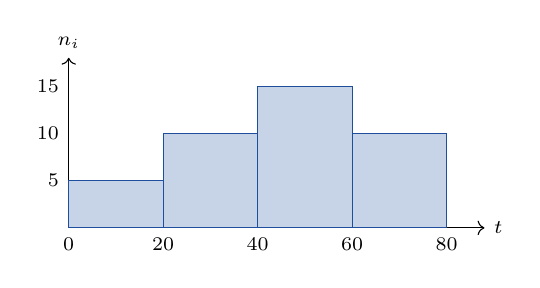
\begin{tikzpicture}[x=0.06cm,y=0.12cm,font=\scriptsize]
\draw[->] (0,0)--(88,0) node[right]{$t$}; \draw[->] (0,0)--(0,18) node[above]{$n_i$};
\foreach \a/\h in {0/5,20/10,40/15,60/10} \draw[fill=cDef!25,draw=cDef] (\a,0) rectangle (\a+20,\h);
\foreach \a in {0,20,40,60,80} \node[below] at (\a,0){$\a$};
\foreach \h in {5,10,15} \node[left] at (0,\h){$\h$};
\end{tikzpicture}\end{LTR}\par}{50 د}{جدول اختيار التمثيل.}
\Row{}{%
\Lab{cThm!80!black}{حذار}\ في المدرج التكراري تكون المساحات متناسبة مع التكرارات ، فننتبه إذا اختلفت أطوال الفئات.}{}{}
\Row{التقويم}{%
\Lab{cEx}{تطبيق}\par في مؤسسة $360$ عاملاً ، $90$ منهم أعمارهم أقل من $30$ سنة. ما زاوية قطاعهم في المخطط الدائري؟\par\textbf{الحل:} $\dfrac{90}{360}\times360^\circ=90^\circ$.\par\textbf{واجب منزلي:} تمارين من الكتاب المدرسي.\par\smallskip\textbf{ملاحظات حول سير الحصة:} \dotfill}{25 د}{تقويم فردي.}
\end{Sayr}
\newpage
\ModhHead{50}{1 ج م ع ت}{إحصاء}{الإحصاء}{02 سا}{مؤشرات الموقع: الوسط الحسابي ، المنوال ، الوسيط}%
{\begin{itemize}\item التوزيعات التكرارية.\end{itemize}}%
{\begin{itemize}\item حساب الوسط الحسابي وخواصه.\item تعيين المنوال والوسيط لسلسلة متقطعة أو مستمرة.\end{itemize}}%
{المنهاج ، الكتاب المدرسي ، مراجع ، الحاسبة العلمية.}
\begin{Sayr}
\Row{مرحلة الانطلاق}{%
\textbf{التهيئة النفسية:} معدلك في الفصل $12$: ماذا يعني ذلك؟ هل هو «أغلب» علاماتك؟}{10 د}{سؤال من حياة التلميذ.}
\Row{التشخيص والاكتشاف}{%
\Lab{cEx}{مناقشة النشاطين 04 و 05 صفحة 140}\par\ck\ فوج من $20$ تلميذاً معدلهم $9$ وفوج من $10$ تلاميذ معدلهم $12$: المعدل العام $\dfrac{20\times9+10\times12}{30}=10$ وليس $\dfrac{9+12}2$.\par
\ck\ نحسب الوسط الحسابي بالتواترات: $\bar x=\sum f_ix_i$.\par
}{35 د}{نكشف خطأ متوسط المتوسطات.}
\Row{بناء المعارف}{%
\Lab{cDef}{تعريف}\par\ck\ \textbf{الوسط الحسابي:} $\bar x=\dfrac{\sum n_ix_i}{N}=\sum f_ix_i$ (لسلسلة مستمرة نستعمل مراكز الفئات).\par
\ck\ \textbf{المنوال:} القيمة (أو الفئة) ذات أكبر تكرار.\par
\ck\ \textbf{الوسيط} $Me$: القيمة التي تقسم السلسلة المرتبة إلى قسمين لهما نفس العدد من القيم.\par
\Lab{cThm}{خطية الوسط}\ إذا كان $y_i=ax_i+b$ فإن $\bar y=a\bar x+b$.\par}{50 د}{نقارن الوسط والوسيط.}
\Row{}{%
\Lab{cEx}{مثال}\par\ck\ سلسلة العلامات (المذكرة 48): $\bar x=\dfrac{300}{30}=10$ ؛ المنوال $10$ ؛ $N=30$ والقيمتان $15$ و $16$ في الترتيب تساويان $10$ ، إذن $Me=10$.\par
\ck\ المكالمات: مراكز الفئات $10$ ، $30$ ، $50$ ، $70$: $\bar t=\dfrac{1800}{40}=45$ s ؛ الوسيط في الفئة $[40;60[$: $Me\approx40+\dfrac{20-15}{15}\times20\approx46{,}7$ s.\par
\Lab{cThm!80!black}{حذار}\ الوسط الحسابي يتأثر بالقيم المتطرفة ، والوسيط لا يتأثر بها.}{}{}
\Row{التقويم}{%
\Lab{cEx}{تطبيق}\par أضاف الأستاذ نقطة لكل تلميذ ثم ضرب العلامات في $1{,}5$. ما الوسط الجديد إذا كان القديم $10$ ؟\par\textbf{الحل:} $(10+1)\times1{,}5=16{,}5$.\par\textbf{واجب منزلي:} تمارين من الكتاب المدرسي.\par\smallskip\textbf{ملاحظات حول سير الحصة:} \dotfill}{25 د}{تقويم فردي.}
\end{Sayr}
\newpage
\ModhHead{51}{1 ج م ع ت}{إحصاء}{الإحصاء}{02 سا}{مؤشرات التشتت: المدى ، الانحراف المتوسط ، الانحراف المعياري ، الانحراف الربعي}%
{\begin{itemize}\item مؤشرات الموقع.\end{itemize}}%
{\begin{itemize}\item حساب مؤشرات التشتت وتفسيرها.\item تلخيص سلسلة بالثنائية (الوسط ، الانحراف المعياري).\end{itemize}}%
{المنهاج ، الكتاب المدرسي ، مراجع ، الحاسبة العلمية.}
\begin{Sayr}
\Row{مرحلة الانطلاق}{%
\textbf{التهيئة النفسية:} قسمان لهما نفس المعدل $10$: هل هما متشابهان بالضرورة؟}{10 د}{مقارنة قسمين.}
\Row{التشخيص والاكتشاف}{%
\Lab{cEx}{وضعية مقترحة}\par القسم (أ): علامات كلها بين $9$ و $11$ ؛ القسم (ب): علامات بين $2$ و $18$ ، والوسط $10$ في الحالتين.\par\ck\ الوسط لا يكفي: نحتاج مؤشراً يقيس \textbf{تشتت} القيم حول الوسط.\par
}{35 د}{نقاش جماعي.}
\Row{بناء المعارف}{%
\Lab{cDef}{تعريف}\par\ck\ \textbf{المدى:} أكبر قيمة $-$ أصغر قيمة.\par
\ck\ \textbf{الانحراف المتوسط:} $\dfrac1N\sum n_i|x_i-\bar x|$.\par
\ck\ \textbf{التباين} $V=\dfrac1N\sum n_ix_i^2-\bar x^2$ و\textbf{الانحراف المعياري} $\sigma=\sqrt V$.\par
\ck\ \textbf{الربيعان} $Q_1$ و $Q_3$ ، و\textbf{الانحراف الربعي} $Q_3-Q_1$.\par
\Lab{cEx}{سلسلة العلامات (المذكرة 48)}\par\ck\ المدى $16-4=12$ ؛ الانحراف المتوسط $\dfrac{72}{30}=2{,}4$.\par
\ck\ $V=\dfrac{3288}{30}-10^2=9{,}6$ ، $\sigma\approx3{,}10$.\par
\ck\ $Q_1$ هي القيمة $8$ في الترتيب: $Q_1=8$ ؛ $Q_3$ هي القيمة $23$: $Q_3=12$ ؛ الانحراف الربعي $4$.\par
}{50 د}{نحسب في جدول بأعمدة إضافية ($n_ix_i$ ، $n_ix_i^2$).}
\Row{}{%
\Lab{cRem}{ملاحظات}\ نلخص السلسلة بـ $(\bar x;\sigma)=(10;3{,}1)$ ؛ كلما صغر $\sigma$ كانت القيم متمركزة حول الوسط.\par\Lab{cThm!80!black}{حذار}\ نستعمل الحاسبة (الوضع الإحصائي) للتحقق.}{}{}
\Row{التقويم}{%
\Lab{cEx}{تطبيق}\par السلسلة: $8$ ، $9$ ، $10$ ، $11$ ، $12$. احسب الوسط والمدى والانحراف المعياري.\par\textbf{الحل:} $\bar x=10$ ؛ المدى $4$ ؛ $V=\dfrac{4+1+0+1+4}5=2$ ، $\sigma=\sqrt2\approx1{,}41$.\par\textbf{واجب منزلي:} تمارين من الكتاب المدرسي.\par\smallskip\textbf{ملاحظات حول سير الحصة:} \dotfill}{25 د}{باستعمال الحاسبة.}
\end{Sayr}
\newpage
\ModhHead{52}{1 ج م ع ت}{إحصاء}{الإحصاء}{02 سا}{تذبذب العينات والمحاكاة}%
{\begin{itemize}\item التواترات.\end{itemize}}%
{\begin{itemize}\item ملاحظة تذبذب التواترات من عينة إلى أخرى.\item محاكاة تجربة بسيطة وملاحظة استقرار التواترات.\end{itemize}}%
{المنهاج ، الكتاب المدرسي ، مراجع ، الحاسبة العلمية.}
\begin{Sayr}
\Row{مرحلة الانطلاق}{%
\textbf{التهيئة النفسية:} نرمي قطعة نقدية $10$ مرات: هل نحصل دائماً على $5$ وجوه؟}{10 د}{تجربة حية.}
\Row{التشخيص والاكتشاف}{%
\Lab{cEx}{مناقشة النشاطين 06 و 07 صفحة 140}\par\ck\ كيس به كريات بألوان مختلفة: كل تلميذ يسحب عينة ويحسب التواترات: النتائج تختلف من عينة إلى أخرى (\textbf{تذبذب العينات}).\par
\ck\ بتجميع عينات القسم (عينة كبيرة) تقترب التواترات من قيم ثابتة.\par
}{35 د}{عمل جماعي بكيس وكريات.}
\Row{بناء المعارف}{%
\Lab{cDef}{تعريف}\ \textbf{العينة} جزء من المجتمع ؛ \textbf{مقاس العينة} عدد عناصرها ؛ \textbf{المحاكاة} تعويض تجربة بتجربة أخرى لها نفس الخواص (قطعة نقدية ، نرد ، أعداد عشوائية بالحاسبة).\par\Lab{cThm}{ملاحظة تجريبية}\ كلما كبر مقاس العينة قلّ تذبذب التواترات واقتربت من قيمة ثابتة.\par}{50 د}{نرسم تطور التواتر مع مقاس العينة.}
\Row{}{%
\Lab{cEx}{مثال}\ محاكاة رمي قطعة نقدية بالحاسبة: نولّد أعداداً عشوائية (الزر \textsc{Ran\#}) ونرفق «وجه» بالعدد إذا كان أقل من $0{,}5$.\par\Lab{cThm!80!black}{حذار}\ النتيجة الملاحظة على عينة صغيرة ليست قاعدة عامة.}{}{}
\Row{التقويم}{%
\Lab{cEx}{تطبيق}\par كل تلميذ يرمي قطعة نقدية $20$ مرة ويسجل تواتر الوجه ، ثم نجمع نتائج القسم. قارن تواتر التلميذ بتواتر القسم.\par\textbf{الحل المنتظر:} تواترات التلاميذ متذبذبة (مثلاً من $0{,}3$ إلى $0{,}7$) ، وتواتر القسم قريب من $0{,}5$.\par\textbf{واجب منزلي:} تمارين حوصلة المحور من الكتاب المدرسي.\par\smallskip\textbf{ملاحظات حول سير الحصة:} \dotfill}{25 د}{نهاية المحور والسنة: فرض أو مراجعة.}
\end{Sayr}
\end{document}
